\documentclass[14pt, a4paper, twoside]{extreport}
\usepackage[utf8]{inputenc}
\usepackage{graphicx}
\usepackage[T2A]{fontenc}
\usepackage{geometry}
\usepackage{array}
\usepackage{graphicx}
\usepackage{setspace}
\usepackage{siunitx}
\usepackage{caption}
\usepackage{titlesec}
\usepackage[russian]{babel}
\usepackage{indentfirst}
\usepackage{setspace}
\usepackage{float}
\usepackage{array}
\usepackage{cellspace}
\usepackage{pgfplots}
\usepackage{pgfplotstable}
\usepackage{tocloft}
\usepackage{amsmath}
\setlength{\cellspacetoplimit}{20pt}
\setlength{\cellspacebottomlimit}{20pt}

\onehalfspacing

\geometry{
  a4paper,
  left=30mm,
  right=20mm,
  top=20mm,
  bottom=20mm
}

\setlength{\parindent}{1.25cm}

\graphicspath{ {images/} }
\captionsetup[figure]{
  labelsep=period,
  justification=centering
}

\renewcommand{\figurename}{Рисунок}
\renewcommand{\contentsname}{\centering Оглавление}

\titleformat{\chapter}[block]{\huge\bfseries\centering}{}{1em}{}
\titleformat{\section}[block]{\normalsize\bfseries}{\thesection}{1em}{}
\titleformat{\subsection}[block]{\normalsize\bfseries}{\thesubsection}{1em}{}
\titlespacing*{\section}{0pt}{\parskip}{-\parskip}
\titlespacing*{\subsection}{0pt}{\parskip}{-\parskip}
\titlespacing{\chapter}{0pt}{0pt}{0pt}

\renewcommand{\cftbeforetoctitleskip}{-30pt}
\renewcommand{\cftaftertoctitleskip}{-10pt}

\begin{document}

\begin{titlepage}
  \begin{center}
    \small
    \underline{
      \begin{minipage}{0.2\textwidth}
        \centering
        
\includegraphics[width=3cm]{BMSTU logo}
      \end{minipage}
      \hfill
      \begin{minipage}{0.8\textwidth}
        \begin{center}

          \textbf{Министерство науки и высшего образования Российской Федерации
            Федеральное государственное бюджетное образовательное учреждение высшего образования «Московский государственный технический университет имени Н.Э. Баумана национальный исследовательский университет»
          (МГТУ им. Н.Э. Баумана)}
        \end{center}
      \end{minipage}

    }

    \vspace{7cm}
    \Large
    \textbf{Лабораторная работа О-107} \\
    "Измерение длины световой волны с помощью колец Ньютона"\\
    \vspace{5cm}
    \normalsize
    \begin{tabular}{p{8cm}p{6cm}}
      \textbf{Студент группы ИУ1-31Б} & \hrulefill \\
      & «\underline{\hspace{1.5cm}}»\underline{\hspace{2.5cm}}2025 г. \\
      & \\
      \textbf{Преподаватель} & \hrulefill \\
      & «\underline{\hspace{1.5cm}}»\underline{\hspace{2.5cm}}2025 г. \\
    \end{tabular}
    \vfill{\Large{Москва, 2025}}
  \end{center}
\end{titlepage}

\tableofcontents
\newpage

\chapter{Конспект}
\section{Цель работы}
Изучить явление интерференции света на установке для наблюдения колец Ньютона, определить радицс кривизны линзы и длину волны света.

\section{Эксперементальное оборудование, приборы и принадлежности}
Лабораторная установка показана на рисунке \ref{pic:labUst}
\begin{figure}[H]
  \begin{center}
    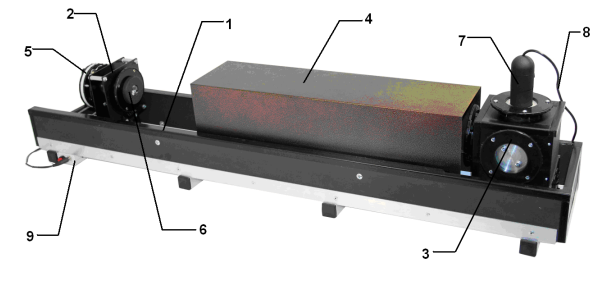
\includegraphics[width=0.8\textwidth]{labUst.png}
  \end{center}
  \caption{}
  \label{pic:labUst}
\end{figure}

Части лабораторной установки :
\begin{enumerate}
  \item Оптическая скамья;
  \item Стойка излучателя;
  \item Оптический бокс;
  \item Сдвижной экран;
  \item Лазерный блок;
  \item Линза;
  \item Цифровой микроскоп расположенный в оптическом боксе;
  \item USB-кабель для чтения данных;
  \item Коммутационный блок.
\end{enumerate}

Оптическая схема установки представлена на рисунке \ref{pic:opticSchema}

\begin{figure}[H]
  \begin{center}
    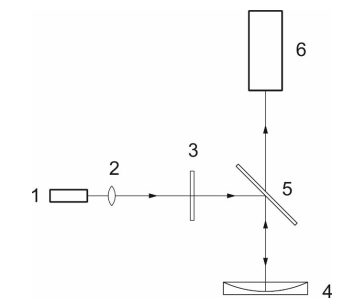
\includegraphics[width=0.7\textwidth]{opticSchema.png}
  \end{center}
  \caption{}
  \label{pic:opticSchema}
\end{figure}

Излучение лазера 1, пройдя через линзу 2, попадает в оптический бокс через входное окно 3, содержащее рассеивающий элемент. Излучение, отраженное от пластины 5, освещает сборку кольца Ньютона 4. Отраженный от нее свет проходит через пластину и попадает на микроскоп 6.

\section{Теоретическая часть}
\subsection{Интерференция}
Сложение двух и более когерентных волн, в результате которого в одних точках пространства происходит увеличение, а в других - уменьшение амплитуды, называется интерференцией.

Когерентные волны - волны с равной частотой и постоянной разностью начальных фаз. Источники таких волн - когерентные источники. Кроме того для наблюдения интерференции необходимо чтобы волны были поляризованы в одной плоскости.

\subsection{Интерференция света при отражении от тонкой пластинки}
Пусть на  прозрачную плоскопараллельную пластинку толщиной $d$ падает под углом $i$ пучок паралленых монохроматических лучей с длиной волны $\lambda$ (рисунок \ref{pic:interference}).

\begin{figure}[H]
  \begin{center}
    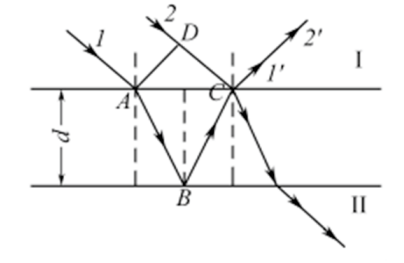
\includegraphics[width=0.6\textwidth]{interference.png}
  \end{center}
  \caption{}
  \label{pic:interference}
\end{figure}
Выделим лучи 1 и 2 этого. Луч 1 после предомления в точке A отражается в точке B и затем после предомленияв точке C интереверирует с отраженным в этой точке лучом 2. Оптическая разность хода лучей в отраженном свете будет равна
\begin{equation}
  \Delta = (AB + BC) n_{\text{пл}} - DC n_{\text{в}} + \lambda/2
\end{equation}
где $n_{\text{пл}}$ - показатель преломления вещества пластинки, а $n_{\text{в}}$ - показатель преломления воздуха, равный 1.

Как следует из рисунка \ref{pic:interference} разность хода можно также выразить через толщину пластинки и угол падения

\begin{equation}
  \Delta = 2d\sqrt{n^2 - \sin^2{i}} + \frac{\lambda}{2}, \quad n = n_\text{пл}
  \label{eq:raznHoda}
\end{equation}

Условия интерференционного минимума(максимума)
\begin{align}
  \Delta &= (2k)\frac{\lambda}{2} \text{- условие максимума}; \\
  \Delta &= (2k+1)\frac{\lambda}{2} \text{- условие минимума};
\end{align}

В проходящем свете оптическая разность хода отличается от оптической разности для отраженного света на $\lambda/2$.Следовательно, максимумам интерференции в отраженном свете соответствуют минимумы интерференции в проходящем свете и наоборот.

\section{Кольца Ньютона}

Если линзу с малой кривизной поместить близко к плоской стекляянной пластине (рисунок \ref{pic:newtonsCircles}), то между линзой и пластиной около точки соприкасновения образуется воздушный клин.

\begin{figure}[H]
  \begin{center}
    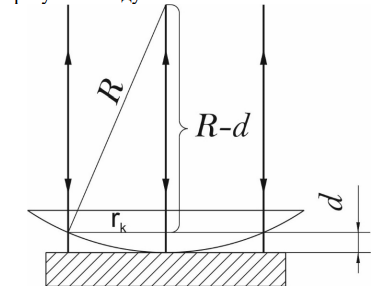
\includegraphics[width=0.6\textwidth]{newtonsCircle.png}
  \end{center}
  \caption{}
  \label{pic:newtonsCircles}
\end{figure}

Линза освещвается лучами, падающими нормально к поверхности воздушного клина. Лучи отраженные от поверхности линзы и пластины когерентны, поэтому они интерферируют. Интерференционные полосы, возникающие при этом имеют вид окружностей (рисунок \ref{pic:circles}).

\begin{figure}[H]
  \begin{center}
    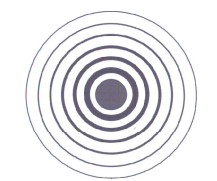
\includegraphics[width=0.3\textwidth]{circles.png}
  \end{center}
  \caption{}
  \label{pic:circles}
\end{figure}

Такие кольца называются кольцами Ньютона. В центре находится темное пятно(минимум нулевого порядка). Оно окружено системой колец ширина и интенсивность которых убывают при удалении от центра.

\subsection{Рассчет радиуса темных и светлых колец интерференционной картины}
Условие (\ref{eq:raznHoda}) запишется в этом случае:

\begin{equation}
  \Delta = 2d + \lambda/2
\end{equation}
где пока преломления воздуха равен единице, а член $\lambda/2$ указывает сдвиг на $\pi$  при отражении света.

Светлые кольца соответствуют толщинам воздушной прослойки $d$, для которых

\begin{equation}
  \Delta = 2d + \frac{\lambda}{2} =  2k\frac{\lambda}{2}, \qquad k=1,2,\dots
  \label{eq:whiteCircle}
\end{equation}

Для темных колец

\begin{equation}
  \Delta = 2d + \frac{\lambda}{2} = (2k+1)\frac{\lambda}{2}, \qquad k=0,1,2,\dots
  \label{eq:blackCircle}
\end{equation}

Из рисунка \ref{pic:newtonsCircles} видно, что радиус кольца Ньютона $r_k$, радиус кривизны линзы $R$ и толщина воздушной прослойки $d_k$ связаны соотношением
\begin{equation}
  r_k^2 = R^2 - (R - d_k)^2
\end{equation}
что эквивалентно
\begin{equation}
  r_k^2 \approx 2Rd_k
  \label{eq:circleRadius}
\end{equation}

Из (\ref{eq:whiteCircle}) выразим $d_k$
\begin{equation}
  d_k = (2k - 1) \frac{\lambda}{4}
\end{equation}

Отсюда
\begin{equation}
  r_k^2 = (2k -1)\frac{\lambda R}{2}
\end{equation}

Таким образом радиус светлых колец равен

\begin{equation}
  r_k = \sqrt{(2k -1)\frac{\lambda R}{2}}
\end{equation}

Аналогично для темных колец

\begin{equation}
  r_k^2 = k\lambda R
\end{equation}

\begin{equation}
  r_k = \sqrt{k\lambda R}
\end{equation}

\subsection{Кольца Ньютона при наличии зазора между линзой и пластинкой}

Толщина воздушного слоя в таком случае равна $d + a$. Тогда оптическая разность хода равна :
\begin{equation}
  \Delta = 2(d + a) + \lambda/2 = 2d + 2a + \lambda/2
  \label{eq:realNewtonCircle}
\end{equation}

Из (\ref{eq:realNewtonCircle}) следует что центр картины  в зависимости от зазора $a$ может быть как светлым так и темным.

\begin{figure}[H]
  \begin{center}
    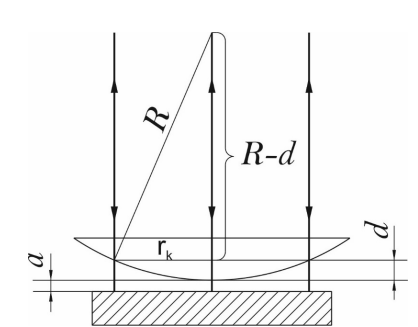
\includegraphics[width=0.6\textwidth]{realNewtonsCircles.png}
  \end{center}
  \caption{}
  \label{pic:realNewtonCircles}
\end{figure}

Разности хода примут следующий вид:
Для светлых колец:
\begin{equation}
  \Delta = 2(d + a) + \frac{\lambda}{2} = 2k\frac{\lambda}{2}, \qquad k=1,2,\dots
\end{equation}

Для темных колец:
\begin{equation}
  \Delta = 2(d + a) + \frac{\lambda}{2} = (2k+1)\frac{\lambda}{2}, \qquad k=0,1,2,\dots
\end{equation}

Найдем $d_k$ для темных колец
\begin{equation}
  2(d_k + a) + \frac{\lambda}{2} = (2k + 1)\frac{\lambda}{2}
\end{equation}
\begin{equation}
  d_k = k\frac{\lambda}{2} - a
\end{equation}

Подставляя в (\ref{eq:circleRadius}) получим
\begin{equation}
  r_k^2 = 2R(k\frac{\lambda}{2} - a) = Rk\lambda - Ra
\end{equation}

Аналогично для светлых колец
\begin{equation}
  d_k = (2k-1)\frac{\lambda}{4} - a
\end{equation}

\begin{equation}
  r_k^2 = 2R((2k-1)\frac{\lambda}{4} - a) = \frac{R\lambda(2k+1)}{2} - 2Ra
\end{equation}

\chapter{Выполнение работы}
\section{Результаты экспериментов}
В результате измерений были получены следующие графики:
\begin{figure}[H]
  \centering
  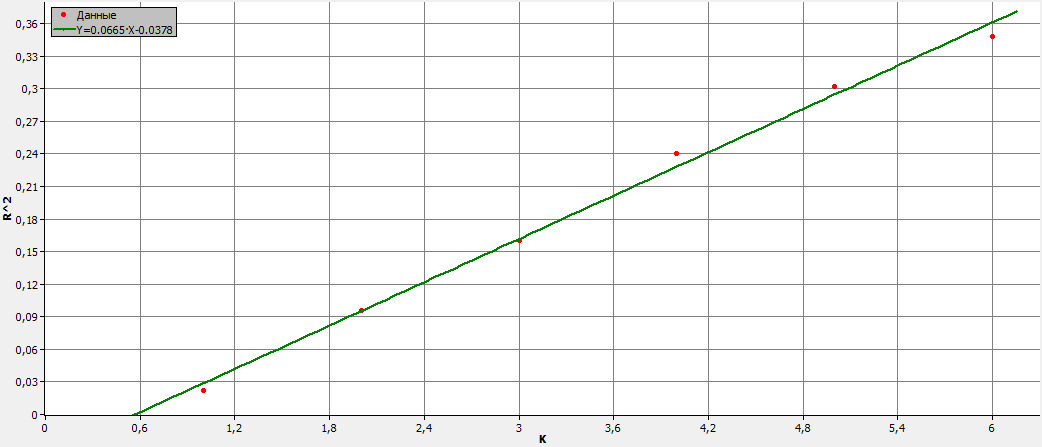
\includegraphics[width=\textwidth]{зеленый граф.jpg}
  \caption{График для зеленого лазера}
\end{figure}

\begin{figure}[H]
  \centering
  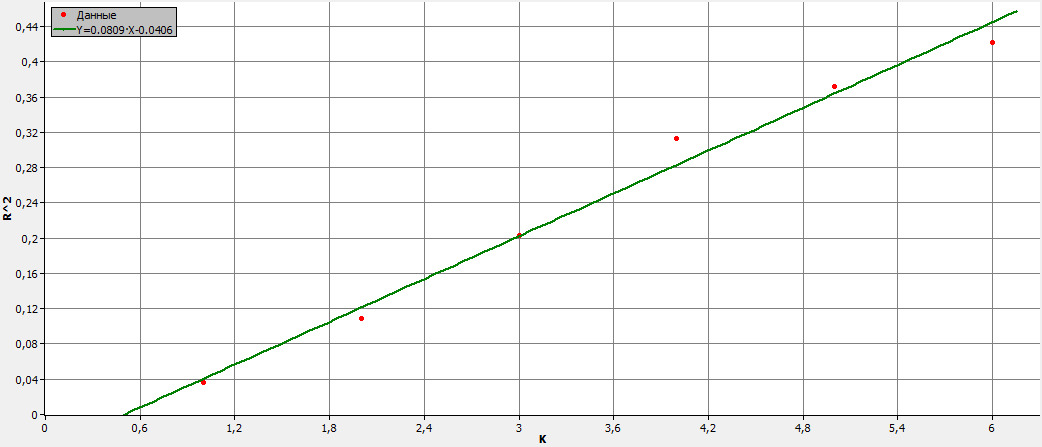
\includegraphics[width=\textwidth]{красный граф.jpg}
  \caption{График для красного лазера}
\end{figure}

Коэффициенты для графика зеленого лазера
\begin{equation}
  \begin{cases}
    A = 0.0665 \text{мм}^2 = 6.65 \cdot 10^{-8} \text{м} ^ 2 \\
    B = -0.0378 \text{мм}^2 = -3.78 \cdot 10^{-8} \text{м} ^ 2
  \end{cases}
\end{equation}

Коэффициенты для графика красного лазера
\begin{equation}
  \begin{cases}
    A = 0.0809 \text{мм}^2 = 8.09 \cdot 10^{-8} \text{м} ^ 2 \\
    B = -0.0406 \text{мм}^2 = -4.06 \cdot 10^{-8} \text{м} ^ 2
  \end{cases}
\end{equation}

\section{Вычисление радиуса кривизны линзы и длины волны красного лазера}

Из теории мы знаем что коэффициент при X равен произведению радиуса кривизны линзы на длину волны, из характеристик лабораторной установки мы знаем что длин волны лазера 515нм. Найдем радиус линзы
\begin{equation}
  r = \frac{A}{\lambda} = \frac{6,65 \cdot 10^{-8}}{515 \cdot 10^{-9}} = 0.1291 \text{м}
\end{equation}

Длина волны красного лазера

\begin{equation}
  \lambda = \frac{A}{r} = \frac{8.09 \cdot 10^{-8}}{0.1291} = 627 \text{нм}
\end{equation}

\section{Вычисление зазора между линзой и пластиной}

Для зеленого
\begin{equation}
  a = \frac{|B|}{2R} = \frac{3.78 \cdot 10^{-8}}{2 \cdot 0.1291} = 0.29 \cdot 10^{-6} \text{м}  = 0.31 \text{мкм}
\end{equation}

Для зеленого
\begin{equation}
  a = \frac{|B|}{2R} = \frac{4.06 \cdot 10^{-8}}{2 \cdot 0.1291} = 0.31 \cdot 10^{-6} \text{м} = 0.31 \text{мкм}
\end{equation}

\section{Вывод}

В ходе лабораторной работы мы исследовали кольца Ньютона для двух источников излучения, Нашли длину волны одного из них, а также радиус кривизны линзны. Научились находить растояние между линзой и пластиной на которой наблюдаются кольца. Выяснили, что это растояние сравнительно мало( < 1 микрометра).

\chapter{Контрольные вопросы}

\begin{enumerate}
  \item \textbf{Что такое интерференция?} \
    Интерференция — это явление наложения двух или более когерентных волн, в результате которого амплитуда результирующей волны в каждой точке пространства зависит от разности фаз исходных волн. Это проявляется в виде периодического изменения интенсивности света.

  \item \textbf{При каком условии можно наблюдать интерференционную картину?} \
    Интерференционная картина наблюдается при наложении когерентных волн, то есть волн с постоянной разностью фаз и одинаковой частотой.

  \item \textbf{Что такое «полосы равной толщины» и «полосы равного наклона»?} \
    \begin{itemize}
      \item Полосы равной толщины — интерференционные полосы, возникающие при изменении толщины слоя между отражающими поверхностями; интенсивность зависит от локальной толщины слоя.
      \item Полосы равного наклона — интерференционные полосы, возникающие при наложении плоских или почти плоских волн; интенсивность зависит от угла падения и наклона поверхностей.
    \end{itemize}

  \item \textbf{Как изменятся радиусы колец, если между линзой и пластинкой налить воду ($n=1.3$)?} \
    Радиусы колец уменьшатся, так как эффективная длина волны в воде уменьшается:
    $
    \lambda_\text{eff} = \frac{\lambda}{n}.
    $

  \item \textbf{Если линза едва касается пластинки, то что наблюдается в центре интерференционной картины?} \
    В центре наблюдается \textbf{темный круг (минимум)} в отражённом свете, так как толщина воздушного слоя равна нулю и разность хода для отражённых волн равна половине длины волны.\
    Чтобы в центре наблюдать поочередно минимум и максимум, необходимо изменить фазовую разность, например, слегка приподняв линзу или изменив длину волны.

  \item \textbf{Каким способом получают когерентные волны для наблюдения колец в отраженном свете?} \
    Когерентные волны получают за счёт отражения от двух поверхностей (линзы и плоскопараллельной пластинки) одной и той же монохроматической волны. Концентрические кольца появляются из-за сферической формы линзы.

  \item \textbf{Почему интерференционная картина имеет вид концентрических колец?} \
    Сферическая форма линзы обеспечивает, что воздушная прослойка между линзой и плоскопараллельной пластинкой изменяется радиально. Это приводит к одинаковой толщине слоя на окружности с центром в точке контакта, формируя концентрические кольца.

  \item \textbf{Как будут выглядеть кольца Ньютона при использовании белого света?} \
    Кольца будут цветными, с радужной окраской. Центр будет темным, так как в нём наблюдается минимум для всех длин волн, а с увеличением радиуса цвета будут меняться.

  \item \textbf{Как изменяются кольца Ньютона при изменении радиуса кривизны линзы, показателя преломления линзы и пластинки?} \
    \begin{itemize}
      \item При увеличении радиуса кривизны линзы радиусы колец увеличиваются.
      \item Увеличение показателя преломления материала линзы или пластинки незначительно изменяет радиусы через фазовую разность, если речь идёт о прохождении света внутри материала.
    \end{itemize}

  \item \textbf{Кольца Ньютона — это полосы «равной толщины» или «равного наклона»?} \
    Кольца Ньютона — это полосы равной толщины.

  \item \textbf{Как изменятся диаметры колец при замене источника монохроматического света на свет с меньшей/большей длиной волны?} \
    \begin{itemize}
      \item При меньшей длине волны диаметры колец уменьшаются.
      \item При большей длине волны диаметры колец увеличиваются.
    \end{itemize}

  \item \textbf{Как изменится интерференционная картина в её центре, если линзу постепенно поднимать над пластинкой?} \
    Центр интерференционной картины постепенно изменится от темного к светлому, так как толщина воздушного слоя увеличивается и разность хода отражённых волн меняется, что приводит к переходу от минимума к максимуму.
\end{enumerate}

\end{document}
